\section*{Aufgabe 2}
\subsection*{a)}
Denken Sie sich eine kleine Sprache aus.
Definieren Sie deren Vokabular mit einer ANTLR4 lexer grammar und deren Grammatik mit einer ANTLR4 parser grammar.
Erzeugen Sie für einige Beispieltexte mit Hilfe von \textit{org.antlr.v4.gui.TestRig} den Ableitungsbaum (Parse Tree).

\subsection*{a - Lösung}
Dargestellt ist der Lexer einer Sprache, welche die korrekte Kreation einer Java Klasse darstellt.
Erlaubt sind Variablen - also einzelne Buchstaben, sowie Zahlen.
Parameter werden durch Komma getrennt und dürfen eigene neu erzeugte Klassen sein.
\newline
\begin{lstlisting}[label={lst:Aufgabe2a_lexer}, style=ANTLR]
    // CreationLexer.g4
    lexer grammar CreationLexer;

    KEYWORD : 'new' ;

    NAME : [A-Za-z]+ ;
    NUM : [0-9]+ ;

    COMMA : ',' ;

    PAR_OPEN : '(' ;
    PAR_CLOSE : ')' ;

    WS : [ \t\r\n]+ ;

    InvalidChar: . ;
\end{lstlisting}

\newpage

Der dazugehörige Parser:
\begin{lstlisting}[label={lst:Aufgabe2a_parser}, style=ANTLR]
    // CreationParser.g4
    parser grammar CreationParser;
    options { tokenVocab=CreationLexer; }

    start : expr EOF;

    expr : KEYWORD WS NAME PAR_OPEN params PAR_CLOSE ;

    params : (param (COMMA WS? param)*)? ;

    param : (expr | NAME | NUM) ;
\end{lstlisting}
\newline

\begin{figure}[h]
    \centering
    \subfloat[\centering Input: new Object(1, 2)]{{ 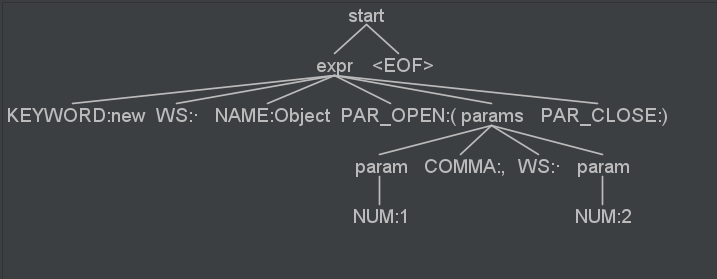
\includegraphics[width=10cm]{images/Aufgabe2a_parseTree_simple} }}
    \qquad
    \subfloat[\centering Input: new Object(1, new Array())]{{ 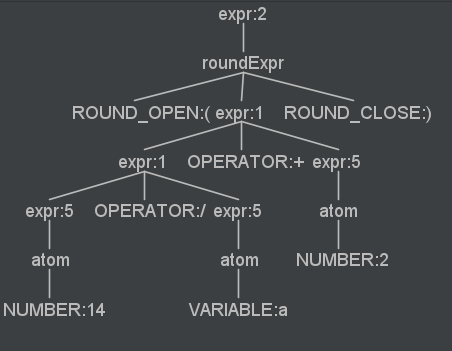
\includegraphics[width=10cm]{images/Aufgabe2a_parseTree} }}
    \caption{Parse Tree Beispiele}
    \label{fig:Aufgabe2a_parseTree}
\end{figure}
\newline

\textbf{Der Parser ist für die grammatikalische Anordnung der durch den Lexer vorgegebenen Token verantwortlich.}
\newpage